\chapter{The Brain}
Amongst the algorithms for choosing the moves in turn-based games, we chose the \textit{alpha-beta pruning} algorithm.
It is a well known algorithm for turn based games, and can be thinked of as an evolution of the basic minimax algorithm, in fact it aims to reduce the number of nodes that are evaluated during the search.

We will discuss the plain minimax algorithm, then the alpha-beta pruning one, and finally the way we used it in our specific case.

\section{Minimax}
\textit{Minimax} is an algorithm for making decisions.
The hipothesis is that of a 2 player zero-sum game, where the outcome goes from -V to V.

One of the player tries to maximize the outcome, while the other tries to minimize it.
For readability sake, we will refer to the two players as to \textbf{Max} and \textbf{Min}.

\textbf{Max} and \textbf{Min} alternate in choosing a move, so each turn consists into two choices, each of which is called a ``ply''.
At each level of the search, the active player watches the outcome associated with each of the options he has, and chooses the one that maximizes his result.
Since the outcome for each of the options depends on the next choice of the other player, the actual choice also minimizes the opponent's result.
This is why the name ``minimax''.\\

\begin{figure}[htbp]
  \centering
    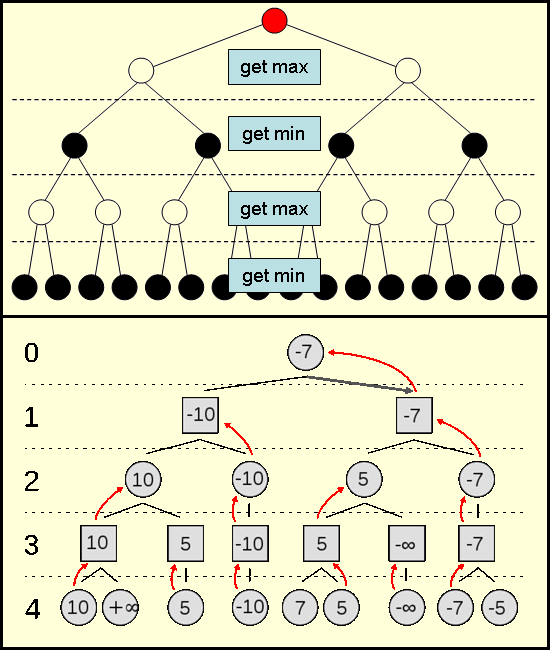
\includegraphics[width=0.5\textwidth]{images/minimax.png}
  \caption{Minimax choosing schema and a simple case example.}
\end{figure}

Of course, when the depth of the tree becomes too high to compute the actual outcome of a choice, we need to use some heuristics. Moreover, this algorithm assumes that the opponent plays with a ``perfect'' strategy, that is reasonable in normal turn-based games, but has some interesting effects when players choose more than a move each time (see chapter \ref{cap:results} for more on this).
